%% LyX 2.1.0 created this file.  For more info, see http://www.lyx.org/.
%% Do not edit unless you really know what you are doing.
\documentclass[english]{article}
\usepackage[T1]{fontenc}
\usepackage[latin9]{inputenc}
\usepackage{geometry}
\geometry{verbose,tmargin=2cm,bmargin=2cm,lmargin=2cm}
\synctex=-1
\usepackage{bm}
\usepackage{amsthm}
\usepackage{amsmath}
\usepackage{graphicx}
\usepackage{setspace}
\usepackage[authoryear]{natbib}
\doublespacing

\makeatletter
%%%%%%%%%%%%%%%%%%%%%%%%%%%%%% Textclass specific LaTeX commands.
\numberwithin{equation}{section}
\numberwithin{figure}{section}

%%%%%%%%%%%%%%%%%%%%%%%%%%%%%% User specified LaTeX commands.
\renewcommand\[{\begin{equation}}
\renewcommand\]{\end{equation}}

\makeatother

\usepackage{babel}
\begin{document}

\title{Beauty Contest}
\maketitle
\begin{abstract}
Pithy, concise and informative. May bring the reader to tears due
to the beauty of it.
\end{abstract}

\section{Introduction}


\section{Methods}

The availability of large data sets for building regression models
to predict the bacterial counts in beach water is both an opportunity
and a challenge. 


\subsection{Data Sources}

\emph{Possibly move this to the end of the section}

Which sites

Where are they

What specific sources sources of data (plug EnDDAT)

Will include a map and tables


\subsection{Listing of specific statistical techniques}

Fourteen different regression modeling techniques were considered.
Each technique uses one of five modeling algorithms: GBM, the adaptive
lasso, the genetic algorithm, PLS, or sparse PLS. Each technique is
aplied to either continuous or binary regression and to either modeling,
or variable selection only.


\subsubsection*{Continuous or binary regression}

The goal of predicting exceednaces of the water quality standard was
approached in two ways: one was to predict the bacterial concentration
and then compre the prediction to a threshold. The other was to predict
the state of a binary indicator, which is coded as zero when the concetration
is below the standard and one when the concentration exceeds the standard.
Techniques taking the former approach are continuous regression techniques,
those taking the latter approach are binary regression techniques.


\subsubsection*{Weighting of observations in binary regression}

A weighting scheme was implemented for some of the binary regression
techniques. In the weighting scheme, observations were given weights
equal to the number of standard deviations the observed concentration
was from the regulatory threshold of 235 CFU/100 mL. Any technique
that was implemented with this weighting scheme was separately implemented
without any weighting of the observations. The techniques are then
labeled weighted and unweighted, respectively.


\subsubsection*{Modeling or selection only}

Some methods are labeled ``select'', which means that they are used
for variable selection only. In these cases, once the variables are
selected, the regression model is estimated using ordinary least squares
for the continuous regression techniques, or ordinary logistic regression
for the binary regression techniques.


\subsubsection{GBM}

GBM refers to the gradient boosting machine (GBM) of \citet{Friedman-2001}.
A GBM model is a so-called random forest model - a collection of many
regression trees. Prediction is done by averaging the outputs of the
trees. Two GBM-based techniques are explored - we refer to them as
GBM and GBMCV. The difference is in how the optimal number of trees
is determined - GBMCV selects the number of trees in a model using
leave-one-out CV, while GBM uses the so-called out-of-bag (OOB) error
estimate. The CV method is much slower (it has to construct as many
random forests as there are observations, while the OOB method only
requires computing a single random forest) but GBMCV should more accurately
estimate the prediction error. All the GBM and GBMCV models share
the following settings:

Number of trees: 10000

Shrinkage parameter: 0.0005

Minimum observations per node: 5

Depth of each tree: 5

Bagging fraction: 0.5


\subsubsection{Adaptive Lasso}

The adaptive lasso \citet{Zou-2006} is a regression method that simultaneously
selects relevant predictors and estimates their coefficients by adding
a penalty to the sum of the squared residuals. For linear regression,
the adaptive lasso estimates $\hat{{\bm{{\beta}}}}$ minimize the
criterion $\sum_{i=1}^{n}(y_{i}-X_{i}\beta)^{2}+\lambda\sum_{j=1}^{p}\frac{{|\beta_{j}|}}{\tilde{{|\beta_{j}|^{\gamma}}}}$,
where $\lambda$ is a tuning parameter and $\tilde{{\bm{{\beta}}}}$
is a consistent estimate of the regression coefficients.

In this work, $\gamma$ is set to one, $\tilde{{\bm{{\beta}}}}$ are
estimated individually by a univariate linear or logistic regression
(it is necessary to estimate the coefficients individually because
there are usually more covariates than observations) and the adaptive
lasso tuning parameter $\lambda$ is selected to minimize the AICc
\citep{Hurvich-Simonoff-Tsai-1998}.

Three of the modeling techniques were based on the adaptive lasso
- one fo


\subsubsection{Genetic algorithm}

The genetic algorithm \citep{Fogel-1998} is a variable-selection
method that works by analogy to natural selection, where so-called
chromosomes represent regression models. A variable is included in
the model if the corresponding element of the chromosome is one, but
not otherwise. Chromosomes are produced in successive generations,
where the first generation is produced randomly and subsequent generations
are produced by combining chromosomes from the current generation,
with additional random drift. The chance that a chromosome in the
current generation will produce offspring in the next generation is
an increasing function of its fitness. The fitness of each chromosome
is calculated by the corrected Akaike Information Criterion (AICc)
\citet{Akaike-1973,Hurvich-Tsai-1989}.

The implementations in this study used 100 generations, with each
generation consisting of 200 chromosomes. The genetic algorithm method
GALM is the default for linear regression modeling in Virtual Beach
\citep{Cyterski-Brooks-Galvin-Wolfe-Carvin-Roddick-Fienen-Corsi-2013}.
The study also investigates two genetic algorithm methods for logistic
regression: one weighted (GALogistic-weighted) and one unweighted
(GALogistic-unweighted).


\subsubsection{PLS}

Partial least squares (PLS) regression is a tool for building regression
models with many covariates \citep{Wold-Sjostrum-Eriksson-2001}.
PLS works by decomposing the covariates into mutually orthogonal components,
with the components then used as the variables in a regression model.
This is similar to principal components regression (PCR), but the
way PLS components are chosen ensures that they are aligned with the
model output. On the other hand, PCR is sometimes criticised for decomposing
the covariates into components that are unrelated to the model's output.

To use PLS, one must decide how many components to use in the model.
The technique used in this study follows the method described in \citet{Brooks-Fienen-Corsi-2013},
using the PRESS statistic to select the number of components.


\subsubsection{SPLS}

Sparse PLS (SPLS) is introduced in \citet{Chun-Keles-2007}. The SPLS
method combines the orthogonal decompositions of PLS with the sparsity
of lasso-type variable selection. To do so, SPLS uses two tuning parameters:
one that controls the number of orthogonal components and one that
controls the lasso-type penalty. The optimal parameters are those
that minimize the mean squared prediction error (MSEP) over a two-dimensional
grid search. The MSEP is calculated by 10-fold cross-validation. Two
techniques utilizing SPLS were 


\subsection{Implementation for beach regression}

The response variable for our continuous regression models is the
natural logarithm of the E. coli concentration. For the binary regression
models, the response variable is 

Include a table with pre/post processing discussion

This includes tuning of parameters

Some specific data issues because we are estimating a threshold exceedence


\subsection{Cross Validation}

Assessment of the modeling techniques is based on their performance
in predicting exceedances of the regulatory standard. Two types of
cross validation was used to measure the performance in prediction:
leave-one-out (LOO) and leave-one-year-out (LOYO). In LOO CV, one
observation is held out for validation while the rest of the data
(the model data) is used to train a model. The model is used to predict
the concentration of that held out observation, and the process is
repeated for each observation. Each cycle of LOYO CV holds out one
year's worth of data for validation instead of a single observation.
It is intended to approximate the performance of the modeling technique
under a typical use case: a new model is estimated before the start
of each annual beach season and then used for predicting exceedances
during the season. That year's data is then added to the dataset to
estimate a model for the next beach season. The LOYO models in this
study were estimated using all the available data, even that from
future years - so for instance the 2012 models were estimated using
the 2010-2011 and 2013 data

Some methods also used cross-validation internally to select tuning
parameters. In those cases the internal CV was done by partitioning
the model data, leaving out one partition at a time. This process
is separate from - and does not affect - the CV to assess predictive
performance.


\subsection{Performance Metrics}

How did we evaluate the performance of each technique on all the different
data sets
\begin{itemize}
\item for all cases ---> AUC (ROC curve)
\item continuous variables using PRESS (skill --> Like Nash-Sutcliffe/R\textasciicircum{}2
over the fitted data) 
\item True/False Positives/Negatives (needs a threshold)
\item Which variables are selected for models where variable reduction takes
place

\begin{itemize}
\item challenge regarding the fact that different variables are selected
in each fold. Maybe use frequencies?
\item also the number of variables selected (metric of complexity)
\end{itemize}
\end{itemize}

\paragraph*{OPTIONAL}
\begin{itemize}
\item AIC/BIC? --> not the same model in each fold so maybe not possible
\item Maybe some form of confusion matrices -- perhaps a grid of them with
or without companion variance plots or other estimates of the range
of results
\end{itemize}

\section{Results}

The area under the ROC (AUROC) curve assesses how accurately the predictions
of the left-out observations are sorted. The methods are ranked at
each site by AUROC and a mean rank (across sites) is computed for
each method. The mean ranks are plotted in 

\begin{figure}
\includegraphics[width=0.45\textwidth]{../figures/LOO-mean-ranks}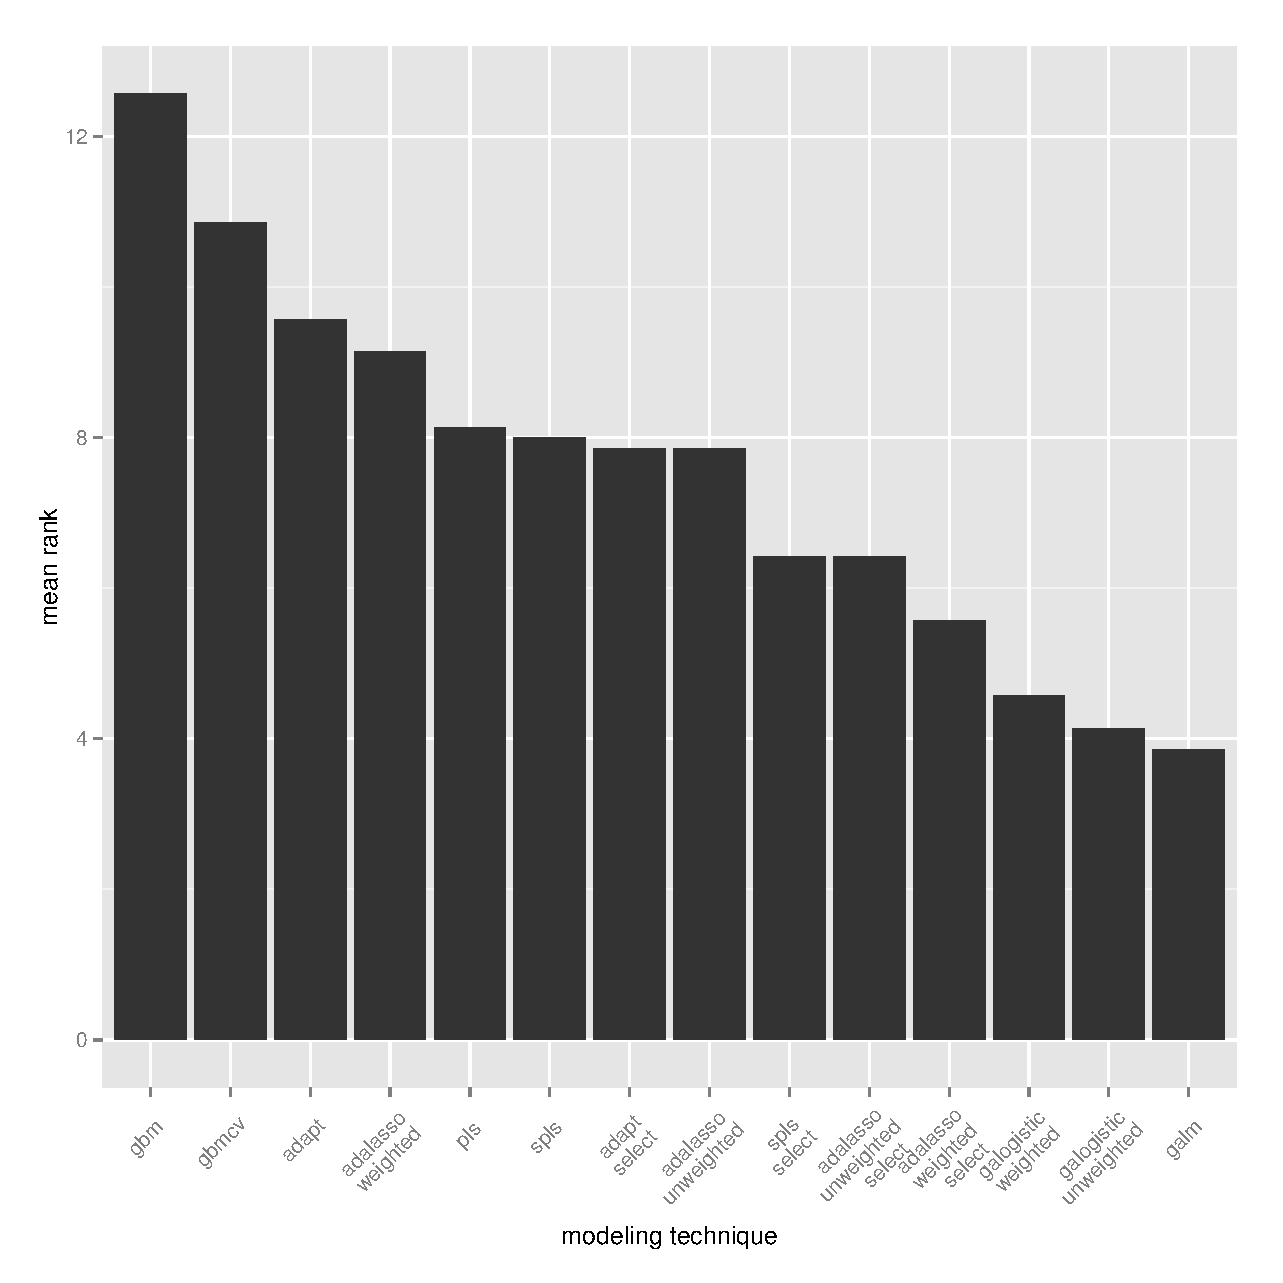
\includegraphics[width=0.45\textwidth]{../figures/LOYO-mean-ranks}

\protect\caption{Mean ranks of the modeling techniques across the seven sites. At left
are the mean ranks under leave-one-out cross validation, at the right
are the mean ranks from leave-one-year-out cross validation.\label{fig:mean-ranks}}


\end{figure}

\begin{itemize}
\item Performance over prediction from cross validation
\item Maybe anecdotal showing fit over data set
\end{itemize}

\section{Discussion}

In general, the GBM, and GBMCV, and AL techniques produced comparable
results that were superior to the other techniques in terms of predictive
performance. Since the GBMCV models take much longer to compute than
the others, we will not include them in our more detailed analysis
of the modeling results.

Which type of model is generally the best?

Under what conditions do some outperform others?

Relative value of overall best model versus methods that help trim
variables? e.g. how valuable is it to reduce number of predictors?
Further, which variables get cut? Expensive ones? Cheap ones?

How important is computational expense? Only an issue for model fitting
--- not prediction, but worth quantifying. E.g. if GBM with cross
validation takes hours, how much better? 

Model tuning for GBM versus GBM-CV --> notes on how GBM is faster
with similar performance (e.g. CV is overkill maybe)


\section{Acknowledgments}


\section{References}

\bibliographystyle{plainnat}
\addcontentsline{toc}{section}{\refname}\bibliography{C:/Users/wrbrooks/git/beauty_contest/references/beautycontest}

\end{document}
